\section{Covariances and Optimal Weights}
Part of scientific computing is statistical computing. If we study how to compute outputs $\hat{x}$ from inputs b, we must also study how to estimate the confidence of $\hat{x}$ from the confidence of b. Confidence is measured by variances and covariances. So we want the covariance
matrix P of the output error (in $\hat{x}$), given the covariance matrix $\Sigma$ of the input error (in b).

The beautiful formula $P=(A^TCA)^{-1}=(A^T\Sigma^-1A)^{-1}$ gives those covariances.
This matrix P shows how reliable or unreliable the estimated x$\hat{x}$ will be. Notice that P
does not depend on a specific b (the experimental data ). It only depends on A and $\Sigma$
(the experimental setup). The knowledge of P tells, in advance, how good the experiment
should be.

This is the “century of data.” Confidence is a central scientific problem. This section goes more deeply into least squares, after the previous section prepared the way with
$A^TA\hat{x}=A^Tb$. The algorithms that lead to $\hat{x}$ connect statistics to other parts of applied mathematics. The analysis of confidence is the crucial link between experiment and simulation.

First we explain variance and covariance. Then we show why the weighting matrix C
(the middle step in our framework) should be the inverse of the input covariance matrix $\Sigma$. Finally we ask how to use new inputs (new measurements) without repeating calculations already done on $b_old$. This is recursive least squares when we are adding new equations in $Au\approx b$. When x and its statistics are changing at each step i, the recursion for $\hat{x}_i$ and its covariance matrix $P_i$ becomes the famous Kalman filter.

	\subsection{Probability Distributions}
	Here are three examples of probability distributions. Example 1 (box-shaped graph) and
	Example 3 (bell-shaped graph) have continuous variables. The height of the curve at the
	point x is the probability density p(x). The chance that a sample falls between x and
	x + dx is p(x)dx. Symmetry of p(x) around zero guarantees that the expected value of
	the error is $m=E\{M\}=0$. Each error is weighted by its probability, and the average is
	zero ( because -x balances out x, when p(-x) = p (x)). Those errors have mean zero.
	
	In Example 2, we count the number of times that M heads appear in N fair coin flips. The number M is a discrete random variable. The probabilities $p_0,...,p_N$ add to 1.
	The expectation $E\{M\}$((the average number of heads) is the mean value N/2. The strong
	law of large numbers says there is zero probability that the fraction M/N will go infinitely often outside a small interval around $\frac{1}{2}$ as we continue to flip the coin.
	
	The normal distribution (the bell-shaped Gaussian) is by far the most common. The
	central limit theorem that averages repeated experiments makes it natural and unavoidable.
	
	Uniform distribution \;Suppose each measurement is rounded to the nearest integer. All
	numbers between 6.5 and 7.5 give 6 = 7. The error e lies between -.5 and .5. All errors in this interval are equally likely (this explains the words uniform distribution).
	
	 The probability that e falls between 0 and $\frac{1}{4}$ is $\frac{1}{4}$:
	 
	 \quad p(x) = 1 \quad Probability that x < error < x + dx is dx
	
	 \quad $\int p(x)dx$ \quad Total probability that$-\frac{1}{2}<e<\frac{1}{2}$ is $\int^{\frac{1}{2}}_{-\frac{1}{2}}dx=1$
	 
	 \quad Mean m \qquad Expected value of the error $E\{e\}=\int^{\frac{1}{2}}_{-\frac{1}{2}}xp(x)dx=0$
	 
	 \quad Variance $\sigma^2$ \quad Expected value of squared error=$\int^{\frac{1}{2}}_{-\frac{1}{2}} x^2 p(x)dx=\frac{1}{12}$
	
	Binomial distribution \; For each flip of a fair coin, the probability of heads is $\frac{1}{2}$.  For N = 3 flips, the probability of heads every time is $\frac{1}{1}^{3}=\frac{1}{8}$. The probability of heads twiceand tails once is $\frac{3}{8}$, from three sequences THH and HTH and HHT. These numbers$\frac{1}{8}$ and $\frac{3}{8}$ are pieces of $(\frac{1}{2}+\frac{1}{2})^{3}=1$:	
	\begin{equation*}
	Total\,probability \quad 
	(\frac{1}{2})^{3}+3(\frac{1}{2})^{3}+3(\frac{1}{2})^{3}+(\frac{1}{2})^{3}=\frac{1}{8}+\frac{3}{8}+\frac{3}{8}+\frac{1}{8}=1
	\end{equation*}
	The average number of heads is 1.5, using those four probabilities as weights:
	\begin{equation*}
	Mean \quad 
	m=(3heads)\frac{1}{8}+(2heads)\frac{3}{8}+(1head)\frac{3}{8}+0=\frac{12}{8}heads
	\end{equation*}
	
	What is the probability of M heads in N flips? Again we look at the terms $(\frac{1}{2}+\frac{1}{2})^{N}$. The chance $p_M$ of seeing M heads and N - M tails involves the binomial coefficient$\begin{pmatrix} N \\ M \end{pmatrix}$= “N choose M” that gamblers know and love:
	\begin{equation*}
	Binomial\, distribution \quad 
	p_M = \frac{1}{2^N}
	\begin{pmatrix}
	N \\ M
	\end{pmatrix}
	=\frac{1}{2^N}\frac{N!}{M!(N-M)!}.
	\end{equation*}
	
	\begin{figure}[h]
		\centering
		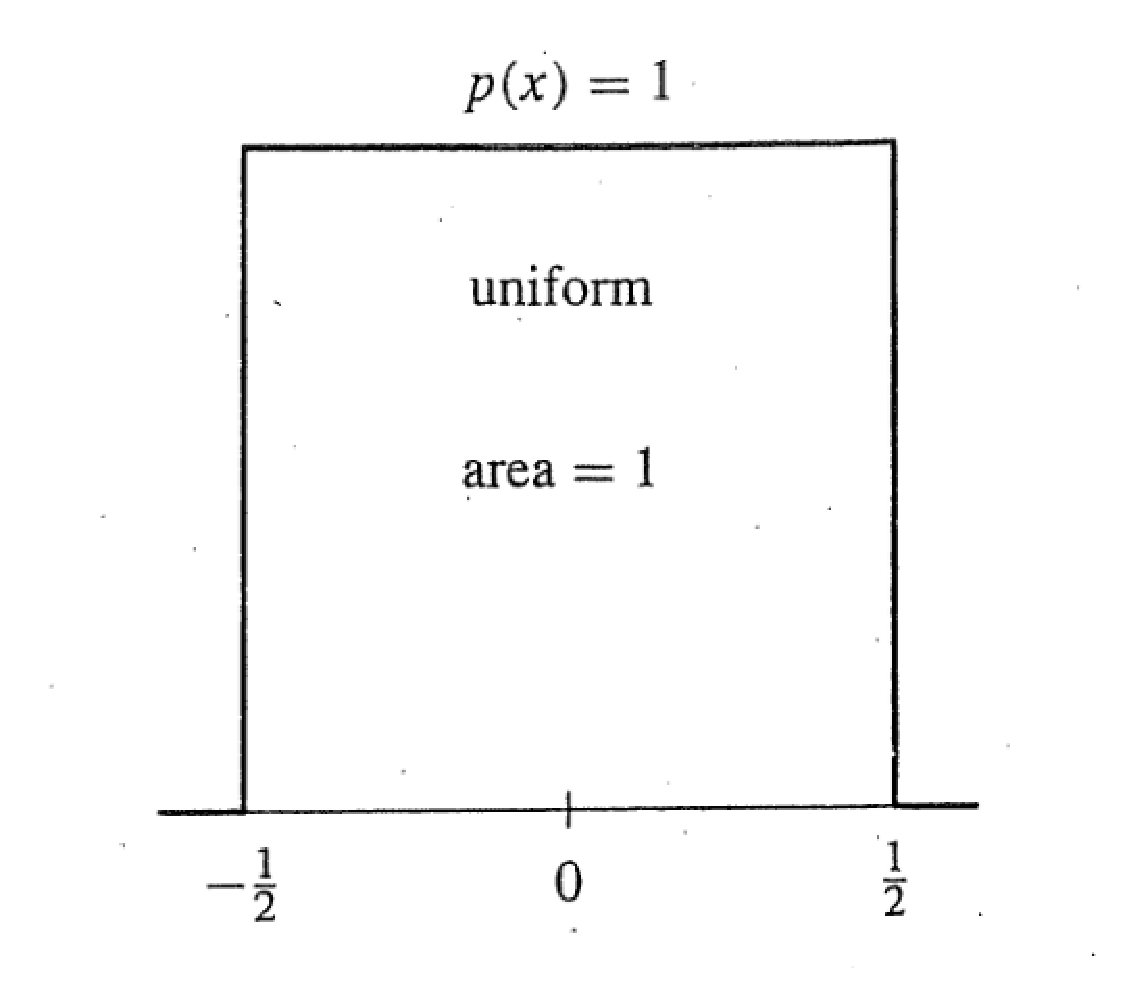
\includegraphics[width=0.7\linewidth]{TeX_files/Part02/chapter04/image/4-2}
		\caption{Figure 4.2 Equal probability between -1/2 and 1/2}
		\label{fig:4-2}
	\end{figure}
	
	The total probability is $p_0+...+p_N=(\frac{1}{2}+\frac{1}{2})^N=1$, see Figure 4.2. The expected
	number of heads is $\bar{M}=0p_0+2p_1+...+Np_N=N/2$. That comes from common sense.
	
	Since the mean is N/2, we work with the squared distance from the mean. Its expected value (squared distance times probability) is the variance $\sigma^2$:
	\begin{equation*}
    Variance \quad 
	\sigma^2=(0-\frac{N}{2})^2p_0 + (1-\frac{N}{2})^2p_1 + ...+ (N-\frac{N}{2})^2p_N
	\end{equation*}
	This turns out to be $\sigma^2=N/4$. The standard deviation is its square root $\sigma=\sqrt{N}/2$.
	This measures the spread around the mean.
	
	An unfair coin has probability p of heads and q = 1 - p of tails. The mean number
	of heads is m = pN. The variance is now $\sigma^2=pqN$.
	
	Normal distribution \; This “Gaussian” distribution is the most important of all. It always
	appears when we combine a large number of identical and independent samples (like coin flips). Normalize the head count M by measuring from the mean N/2 and dividing by the standard deviation $\sigma=\sqrt{N}/2$.
	\begin{equation*}
	Normalized\, count\, of\, heads \quad
	x=\frac{1}{\sigma}(M-mean)=\frac{2}{\sqrt{N}}(M-\frac{N}{2}).
	\end{equation*}
	
	As N increases, the possible outcomes x begin to fill in the whole line from $-\infty$ to $\infty$. The Central Limit Theorem says that the probabilities for these random variables x approach a Gaussian distribution. The probability that the normalized head count falls in the small interval between x and x + dx is
	\begin{equation}
	p(x)dx=\frac{1}{\sqrt{2\pi}}e^{-x^{2}/2}dx \quad
    with\,total\,probability 
	\quad\int^{\infty}_{-\infty}p(x)dx=1.
	\end{equation}
	
	\begin{figure*}[h]
		\centering
		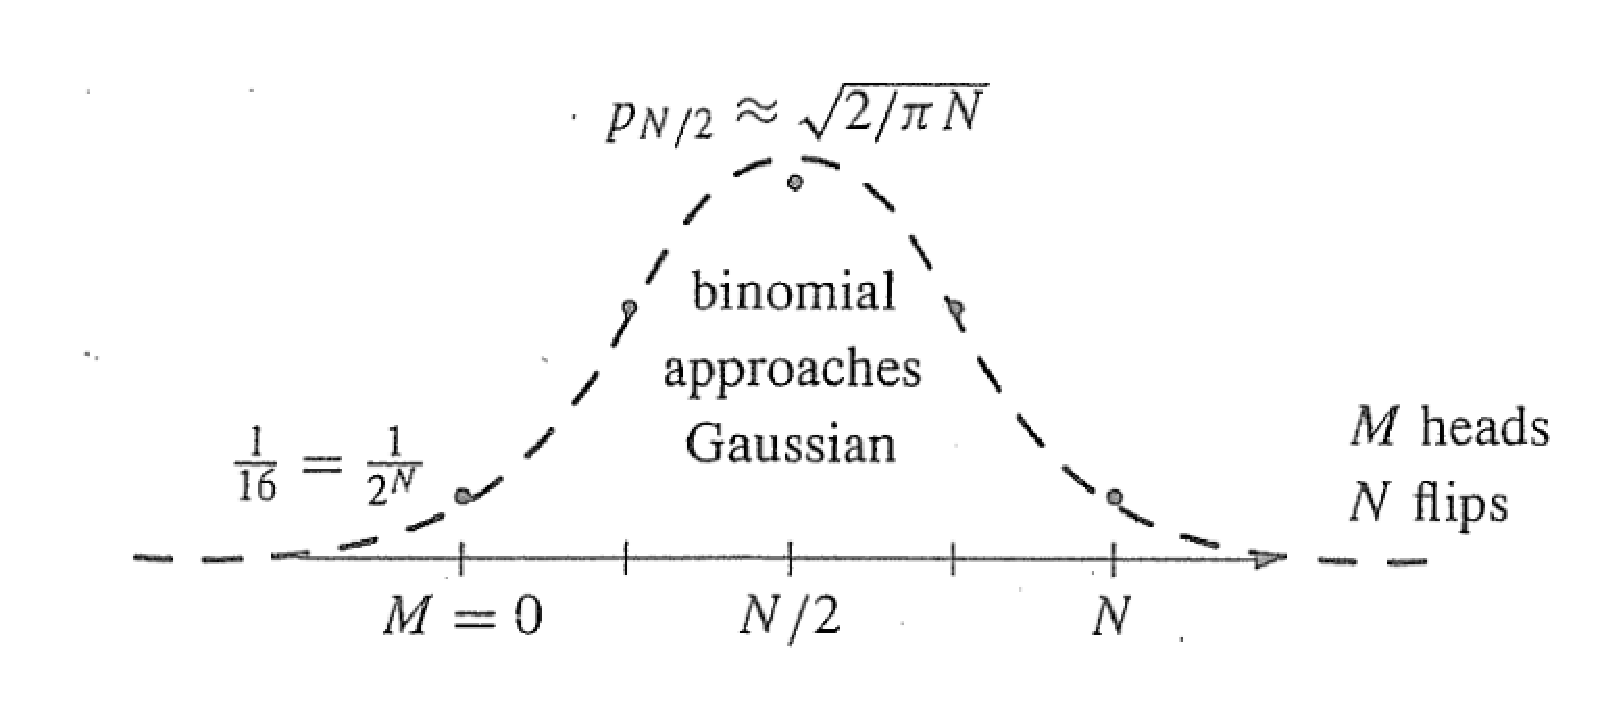
\includegraphics[width=0.7\linewidth]{TeX_files/Part02/chapter04/image/4-3}
		\caption{}
		\label{fig:4-3}
	\end{figure*}
	
	Figure 4.3 \; The binomial distribution p=(1,4,6,4,1)/16 adding to 1 comes from$\begin{pmatrix}
	N \\ M \end{pmatrix}/2^N$ with N = 4. This approaches a Gaussian distribution of height
	$\sqrt{2/\pi N}$ and variance $\sigma^2=N/4$.
	
	The factor $\sqrt{2\pi}$ ensures that the total probability equals one. The graph of $e^{-x^{2}/2}$ is the famous bell-shaped curve in Figure 4.3. Its integral F(x) gives the cumulative
	probability of all outcomes up to but not exceeding x. By symmetry, the mean value
	of x is $\int xp(x)dx=0$. The variance is $\int x^2p(x)dx=1$. MATLAB’s randn uses
	this normal distribution, where the output from rand is uniformly distributed.
	
	This “standard” normal distribution, with mean m = 0 (more often written $\mu=0$) and variance $\sigma^2=1$, was produced by normalizing the head count. A non-standard normal distribution is centered at its mean $\mu=\int xp(x)dx$, and the “width of the bell” is $\sigma$:
	\begin{equation}
	p(x)=\frac{1}{\sqrt{2\pi}\sigma}e^{-(x-\mu)/2\sigma^{2}}
	\quad has \quad
	\int p(x)dx=1 \quad and \quad \int(x-\mu)^2p(x)dx=\sigma^2
	\end{equation}
	 
	 When you read the results of a poll, the newspaper always gives the mean value $\mu$ .
	 Very often it also reports the interval from$\mu-2\sigma$ to $\mu+2\sigma$. The probability is
	 about $95\%$ that the sample lies in this range. You can see from Figure 4.5(where $\Sigma=1$) that about $95\%$ of the area under p(x) lies between $-2\sigma$ and $+2\sigma$. That area is shown by the “cumulative probability” F(x), the integral of p(x). The definite integral F(2)-F(-2) is close to 0.95, the likelihood of errors $<2\sigma$.
	 
	 Multivariate Normal Distribution\; For m random variables, the probability density function moves from p(x) to $p(b)=p((b_1,...,b_m)$. The normal distribution with mean zero was controlled by one positive number $\sigma^2$. Now p(b) is controlled by an m x m positive definite matrix $\Sigma$. This is the covariance matrix and its determinant is $|\Sigma|$:
	 \begin{equation*}
	 p(x)=\frac{1}{\sqrt{2\pi}\sigma}e^{-x^2/2\sigma^2}
	 \quad becomes \quad
	 p(b)=\frac{1}{(2\pi)^{m/2}|\Sigma|^{1/2}}e^{-b^{T}\Sigma^{-1}b/2}
	 \end{equation*}
	
	The integral of p(b) over m-dimensional space is the total probability 1 . The integral
	of bp(b) gives the mean values of $b_1,...,b_m$. Those are all zero. The integral of
	$bb^Tp(b)$gives the covariance matrix E for this multivariate normal distribution. This
	integral reduces to the matrix $\Sigma$ that appears in the exponent.
	
	In case $\Sigma=I$, the exponent $-b^T\Sigma^-1b/2$ is just the sum —$-(b^2_1+...+b^2_m)/2$. So
	the distribution $p(b_1,...b_m)$is the product of the m separate 1-dimensional normal distributions —as we expect when $\Sigma=I$.
	
	Now we need to understand the meaning of covariances $\sigma_ij$ and the matrix $\Sigma$.
	
	\subsection{The Covariance Matrix}
	Run m different experiments at once. They might be independent, or there might be some
	correlation between them. Each measurement x is now a vector, containing the output $x_i$
	from each of the m experiments. We want to say more about covariance.
	
	If we measure distances $e_i$ from the means, each error $e_i$ has mean zero. If two
	errors $e_i$ and $e_j$ are independent (no relation between them), their product $e_ie_j$ also has
	mean zero. But if the measurements are by the same observer at nearly the same time, the
	errors $e_i$ and $e_j$ could tend to have the same sign or the same size. The errors in the m
	experiments could be correlated. Position errors from m neighbouring receivers are very
	likely to be correlated. The average of the product $e_ie_j$ is the covariance $\sigma_ij$:
	\begin{equation}
	Covariance \quad
	\sigma_ij=\sigma_ji=E\{e_ie_j\}=e_i*e_j.
	\end{equation}
	This is the (i,j) and (j, i) entry of the covariance matrix $\Sigma$. The (i,i) entry on the
	diagonal of E $\Sigma$ is the variance of $\sigma^2_i$.
	
	One way to estimate this number $\sigma_ij$ is to run the experiment many times. An opinion
	poll might find that the replies from a wife and husband are correlated. Could be positive,
	could be negative. Replies might tend to be the same (covariance $>$ 0) or possibly opposite
	(covariance $<$ 0). It is an important and nontrivial problem to estimate the variances and
	covariances from the data.
	
	If each experiment is run m times , the output vectors $x^1,x^2,...,x^m$ provide sample means $\bar{\mu_i}$ and sample variances $\bar{\sigma_i}^2$ and covariances$\bar{\sigma_{ij}}$. These are a natural choice when we don't know the true $\mu_i$ and $\sigma^2_i$ and $\sigma_{ij}$:
	\begin{equation}
	Sample \,values \quad
	\bar{\mu_i}=\frac{x^1_i+...+x^m_i}{m}  \qquad \bar{\sigma_ij}=\frac{(x^k_i-\bar{\mu_i})(x^k_j-\bar{\mu_j})}{m-1}.
	\end{equation} 
	Notice the division by m - 1, when “one degree of freedom is used” in $\mu_i$.
	
	Example 4.2\; Let m observations of the same scalar variable x be given as $b_1,...,b_m$. We
	want to prove that the weighted mean $\hat{x}$ and its variance are given as
	\begin{equation}
	\hat{x}=\frac{u^TCb}{u^TCu} 
	\quad and \quad 
    \hat{\sigma}^{2}_{\hat{x}}=\frac{1}{(m-1)}\frac{\hat{e}^TC\hat{e}}{u^TCu}.
	\end{equation}
	Here we introduced $\hat{e}=b-A\hat{x}$ and the vector $u^T=[1 1 ... 1]$. The m observation
	equations $x_i=b_i-e_i$ can be written in the matrix form Ax = b - e with A = u:
	\begin{equation*}
	\begin{bmatrix}
	1 \\ 1 \\ \vdots \\1
	\end{bmatrix}
	x=
	\begin{bmatrix}
	b_1 \\ b_2 \\ \vdots \\ b_m
	\end{bmatrix}
	-
	\begin{bmatrix}
	e_1 \\ e_2 \\ \vdots \\ e_m
	\end{bmatrix}
	\end{equation*}
	The normal equations $A^TCAx=A^TCb$ are
	\begin{equation*}
	\begin{bmatrix}
	1 & \dots & 1
	\end{bmatrix}
	\begin{bmatrix}
	c_1 & \quad  &\quad \\
	\quad & \ddots & \quad \\
	\quad & \quad  & c_m
	\end{bmatrix}
	\begin{bmatrix}
	1 \\ \vdots \\ 1
	\end{bmatrix}
	\hat{x}=
	\begin{bmatrix}
	1 & \dots & 1
	\end{bmatrix}
	\begin{bmatrix}
	c_1 & \quad  &\quad \\
	\quad & \ddots & \quad \\
	\quad & \quad  & c_m
	\end{bmatrix}
	\begin{bmatrix}
	b_1 \\ \vdots \\ b_m
	\end{bmatrix}.
	\end{equation*}
	This is $\Sigma^{m}_{i=1}c_i\hat{x}=\Sigma^{m}_{i=1}c_ib_i$ and the solution is the weighted mean $\hat{x}$:
	\begin{equation}
	\hat{x}=\sum_{i=1}^{m}c_ib_i / \sum_{i=1}^{m}c_i=u^TCb/u^TCu
	\end{equation} 
	
	Example 4.3\; Finally we make a preliminary inspection of the concept of correlation and
	its eventual influence. Suppose we have observed a given distance twice, with the results
    $b_1=100m$ and $b_2=102m$. The least-squares estimate for the length is $\hat{x}$. If C = I then
	$\hat{x}=101m$ is the average. In case C is diagonal we get $b_1<\hat{x}<b_2$. When $c_1\textrightarrow \infty$ we approach $\hat{x}=b_1$ and when $c_2\textrightarrow \infty$ we obtain $\hat{x}=b_2$. The least-squares result for diagonal C (no correlation) always lies between the smallest and the largest observation.
	
	If the two observations are correlated the circumstances change drastically. We still
	have$A^T=\begin{bmatrix} 1 & 1\end{bmatrix}$ for the two observations. Suppose the inverse covariance matrix is
	\begin{equation*}
	\begin{bmatrix}
	5 & 2 \\ 2 & 1
	\end{bmatrix}^{-1}
	=
	\begin{bmatrix}
	1 & -2 \\ -2 & 5
	\end{bmatrix}
	=C
	\end{equation*}
	Now $A^TCA=2$ and $A^TCb=206$. Therefore $\hat{x}=103>b_2$. A strong positive correlation
	combined with a large weight for $b_2$ results in $\hat{x}>b_2$ which cannot happen for independent observations. In Section 6.5 we shall show how arbitrary covariance matrices may lead to arbitrary least-squares results. You may run the M-file corrdemo.
	
	Suppose we know the true joint distribution of two errors. This is the probability
	p(x,y)dxdy that $e_1$ lies between x and x + dx and	$e_2$ lies between y and y + dy. Then a
	double integral over all x and y gives the covariance of the errors. When the means $\bar{x}$ and $\bar{y}$ are not zero, replace x and y by $x-\bar{x}$ and $y-\bar{y}$:
	\begin{equation}
	Covariance \quad
	\sigma_12=\iint xyp(x,y)dxdy
	\end{equation}
	For independent errors, p (x,y) is the product p(x)p(y). The double integral is $\sigma_12=0$:
	\begin{equation*}
	Independence \quad
	\sigma_12=\iint xyp(x)p(y)dxdy=\int xp(x)dx\int yp(y)dy=(0)(0)
	\end{equation*}
	Covariances are zero and $\Sigma$ becomes a diagonal matrix, when e's are independent. This
	case is computationally the easiest by far.
	
	The diagonal entries of $\Sigma$ are the variances $\sigma^2$. Those are the averages of $e^2_i$, necessarily positive. There is a neat way to put all variances and covariances into one matrix formula , using the column vector e times the row $e^T$:
	\begin{equation}
	Covariance \,matrix \quad
	\Sigma=E\{ee^T\}=E
	\begin{Bmatrix}
	e^2_1 & e_1e_2 & \quad & e_1e_m \\
	\quad &\quad   & \dots & \quad  \\
	e_me_1&e_me_2  & \dots &e^2_m
	\end{Bmatrix}
	\end{equation}
	The average value of that product $ee^T$ is $\Sigma$. This matrix is always symmetric and almost
	always positive definite! (It is semidefinite when a fixed combination of the errors is zero
	all the time. That indicates a poor experiment.) The key step coming next is to show that
	C should be chosen as $\Sigma^{-1}$.
	
	The “correlation coefficient” is a dimensionless (scaled) form $p_{ij}=\sigma_{ij}/\sigma_i\sigma_j$ of the covariance. The diagonal entries of the correlation matrix are $\sigma^2/\sigma^2=1$.
	
	\subsection{The Weighting Matrix $C=\Sigma^{-1}$}
	We will show that the choice $C=\Sigma^{-1}$ minimizes the expected squared error in $\hat{x}$. Start with the normal equation for $\hat{x}$, which produces the matrix L in $\hat{x}=Lb$:
	\begin{equation}
	A^TCA\hat{x}=A^TCb
	\quad give \quad
	\hat{x}=(A^TCA)^{-1}A^TCb=Lb
	\end{equation}
	Notice that L times A, which is $(A^TCA)^{-1}A^TC$ times A, gives LA = I.
	
	We want the covariance matrix (all the variances and covariances) for the output
	error vector $x-\hat{x}$. Since LA = I and $\hat{x}=Lb$ this output error is -Le:
	\begin{equation}
	Output error \quad
	x-\hat{x}=LAx-Lb=-L(b-Ax)=-Le
	\end{equation}
	m equation (4.16), the matrix $ee^T$ produced all the products $e_ie_j$. Similarly we multiply a
	column $x-\hat{x}$ times its transpose to get an n by n matrix. The covariance matrix P for the
	error $x-\hat{x}$ is the average value (expected value) of $(x-\hat{x})(x-\hat{x})^T$:
	\begin{equation}
	Covariance \quad
	P=E\{(x-\hat{x})(x-\hat{x})^T\}=E\{(Le)(Le)^T\}=LE\{ee^T\}L^T=L\Sigma L^T
	\end{equation}
	This is our key equation. The second step uses (4.18). The only new step was to bring the
	constant matrices L and $L^T$ outside the sums or integrals for the expected value $E\{ee^T\}$.
	That is standard procedure, and it is called “propagation of variance.” Now we are ready
	to minimize P, by choosing the best C in this matrix L. Here is the result.
	
	Under the requirement LA = I, the covariance matrix $P=L\Sigma^{-1}L^T$ is as small as
	possible when C (the matrix used in L) is $C=\Sigma^{-1}$. This gives the best linear unbiased
	estimate $\hat{x}$( BLUB ). The covariance matrix P for the errors $x-\hat{x}$ simplifies to
	\begin{equation}
	Output\, covariances\, when\, C=\Sigma^{-1} \quad
	P=E\{(x-\hat{x})(x-\hat{x})^T\}=(A^T\Sigma^{-1}A)^{-1}
	\end{equation}
	To check (4.20), use $C=\Sigma^{-1}$ in the matrix L. This choice gives a special $L=L^*$:
	\begin{equation}
	P=L^*\Sigma L^{*T}=((A^T\Sigma^{-1}A)^{-1}A^T\Sigma^{-1})\Sigma(\Sigma^{-1}A(A^T\Sigma^{-1}A))=(A^T\Sigma^{-1}A)^{-1}
	\end{equation}
	A different choice of C gives a different L. We still have LA = I and $L^*A=I$, so $(L-L^*)A=0$.
	To show that the change away from $C=\Sigma^{-1}$ produces a larger covariance matrix P, write $L=L^*+(L-L^*)$. Computer $P=L\Sigma L^T$ or this different choice:
	\begin{equation}
	P=L^*\Sigma L^{*T} + (L-L^*)\Sigma L^{*T} + L^*\Sigma(L-L^*)^T + (L-L^*)\Sigma(L-L^*)^T
	\end{equation}
	The middle terms in (4.22) are transposes of one another, and they are both zero:
	\begin{equation}
	(L-L^*)\Sigma(\Sigma^{-1}A(A^T\Sigma^{-1}A)^{-1})=(LA-L^*A)(A^T\Sigma^{-1}A)^{-1}=0
	\end{equation}
	The last term in (4.22) is positive semidefinite. That term is zero and P is smallest when
	$L=L^*$, now proved to be the best. Then the inverse matrix $P^{-1}=A^T\Sigma^{-1}A$ is called the	information matrix. It goes up as $\Sigma$ goes down (better observations). It also goes up as the experiment continues. Adding new rows to A increases $A^T\Sigma^{-1}A$.
	
	Remark 4.1\; We can obtain $\Sigma=I$(whiten the noise) by a change of variables. Factor
	$\Sigma^{-1}$ into $W^TW$ and introduces $\epsilon=We$. These normalized errors W(b - Ax) have
	$\Sigma=I$:
	\begin{equation*}
	Normalized \,covariance \quad
	E\{\epsilon\epsilon^T\}=WE\{ee^T\}=W\Sigma W^T=I
	\end{equation*}
	This weighting returns us to white noise, $\sigma^2_i=1$and$\sigma_{ij}=0$. Ordinary least squares.
		
	Remark 4.2\; We can always obtain $C=I$ from $C=\sigma^2_0\Sigma^{-1}_b$ by a change of variables.
	Factor the matrix $\sigma^2_0\Sigma^{-1}_b$ into $W^TW$ and introduce $\bar{e}=We$. (Often W is denoted $\sigma^2_0\Sigma^{-1/2}_b$, we matrix square root of $\Sigma^{-1}_b$.) These standardized errors $\bar{e}=W(b-Ax)$ still have mean zero, and their covariance matrix is the identity:
	\begin{equation*}
	E\{(We)(We)^T\}=WE\{ee^T\}W^T=W\Sigma_bW^T=I
	\end{equation*}
	The weighting matrix W returns us to white noise — a unit covariance problem, with simpler theory and simpler computations.*
	
	Remark 4.3 \;If one of the variances is zero, say $\sigma^2_1=0$, then the first measurement is
	exact. The first row and column of $\Sigma_b$ are zero, and $\Sigma_b$ is not positive definite or even invertible. (The weighting matrix has $(\Sigma^{-1}_b)_{11}=\infty$.) This just means that the first equation in Ax = b should be given infinite weight and be solved exactly. If this were true of all m measurements we would have to solve all m equations Ax = b, without the help of least squares; but with exact measurements that would be possible. 
	